\section{Introduction}

The \emph{Hecke algebra} $H_W(q)$ associated to a Coxeter group $W$ is, loosely speaking, a $q$-deformation of the group algebra of $W$. It is defined via a set of generators $T_w$ for each $w\in W$, with relations inherited from the Coxeter group $W$. The seminal work of Kazhdan and Lusztig \cite{KL79} showed that, $H_W(q)$ admits a different basis $\{C_w\}$ which better controls the representation theory of $H_W(q)$. 

The Schur Weyl duality between a Weyl group $W$ and a Lie algebra $\mathfrak{g}$, extend to a duality between the Hecke algebra $H_W(q)$ and the $q$-deformed universal enveloping algebra $U_q(\mathfrak{g})$ (quantum group). The KL basis $\{C_w\}$, under the Schur-Weyl duality, is exactly Lusztig's canonical basis for quantum groups. In other words, the KL basis is the ``canonical basis'' for $H_W(q)$. The canonical basis was independently discovered (dually?) by Kashiwara under the name of global basis. Taking modulo $q$, it specializes to the \emph{crystal basis}, which has rich combinatorial properties.

Alternatively, considering vector space dual of the quantum group, we have the \emph{dual canonical basis} of the quantized coordinate ring. To study elements of dual canonical basis, Fomin and Zelevinsky introduced \emph{cluster algebras}\footnote{a combinatorial ``machine'' designed to produce elements of dual canonical basis}, which has now grown to a important area of research of its own.

A \emph{Coxeter system} is a pair $(W,S)$, where $W$ is the \emph{Coxeter group} and $S$ is the set of simple generators, satisfying relations like
\[
s_i^2=1,\quad
(s_is_j)^{m_{ij}}=1	
\]for some positive integers $m_{ij}$. Our main example will be the symmetric group $\sn$. The \emph{reduced expression} of $w\in W$ is the minimal way to write $w$ in terms of simple generators: $w=s_{a_1}\cdots s_{a_l}$. This leads to the notion of \emph{length} of $w$, denoted $\ell(w)$, that is the number of $s_i$'s in the reduced expression of $w$. For example, in $\mathfrak{S}_3$, we have $321=s_1s_2s_1=s_2s_1s_2$, and $\ell(321)=3$.
The subword order on reduced expressions is called the \emph{Bruhat order} on $W$. For example, the Hasse diagram of the Bruhat order of $\mathfrak{S}_3$ is the follows.
\begin{center}
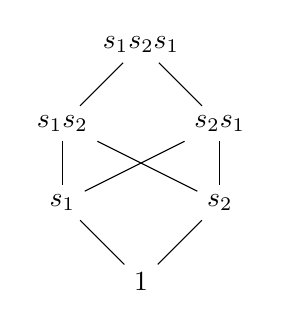
\begin{tikzpicture}
	\node (321) at (0,3) {$s_1s_2s_1$};
	\node (213) at (-1,1) {$s_1$};
	\node (132) at (1,1) {$s_2$};
	\node (123) at (0,0) {$1$};
	\node (231) at (1,2) {$s_2s_1$};
	\node (312) at (-1,2) {$s_1s_2$};
	\draw (321) --(231)--(213) -- (123) --(132)--(312)--(321);
	\draw (213) --(312);
	\draw (132)--(231);
	 \end{tikzpicture}	
\end{center}

The Hecke algebra $H_W(q)$ of a Coxeter group $W$ is generated by a set of generators $\{T_w\}$, for each $w\in W$. They satisfy the following relations.
\[\begin{cases}
T_sT_w =T_{sw}&\text{if }\ell(sw)>\ell(w)\\
T_s^2 = (q-1)T_s+qT_1	
\end{cases}
\]
where $q$ is a formal parameter. It can been seen that $H_W(q)$ is a $q$-deformation of the group algebra of $W$, by setting $q\mapsto 0$.

One may ask what are the inverses of these $T_w$'s. The answer of this question leads to the following theorem/definition.
\begin{theorem}[KL?]There exists a family of polynomials $R_{v,w}(q)$ for every $v,w\in W$, such that
\[(T_w)^{-1}=q\sum_{x\leq w}R_{xw}(q) T_x\]	
These polynomials $R_{v,w}(q)$ are called \emph{the $R$-polynomials}.
\end{theorem}
The Hecke algebra $H_W(q)$ has an automorphism $\eta$ (an involution) defined as follows.
\begin{align*}
q&\mapsto q^{-1}\\	
T_w&\mapsto (T_{w^{-1}})^{-1}
\end{align*}
We want a new basis $\{C_w\}$ for $H_W(q)$ such that 
\begin{enumerate}
	\item $C_w$ is a linear combination of $T_x$ for $x\leq w$.
	\item $\eta(C_w)=C_w$
	\item coefficients of $C_w$ (as in (1)) are ``as simple\footnote{being simple means it's a polynomial whose degree is not too big.} as possible''.
\end{enumerate}

It turns out that the KL basis is the unique one satisfying these properties, which makes it ``canonical''. [Ben asked the geometric meaning of 
canonicity, fill in later.]
\begin{theorem}[KL]
	There exists a unique family polynomials $P_{x,w}(q)$ for each $x\leq w\in W$ such that
	\[C_w'=q^{\cdots} \sum_{x\leq w}P_{x,w}(q)T_x\]
	These polynomials are called \emph{Kazhdan-Lusztig polynomials} and can be computed recursively.
\end{theorem}
%KL polynomials are notoriously hard to compute, and patterns about then are usually hard to believe. 

It is promised that Kazhdan-Lusztig polynomials give rise to beautiful combinatorics. One example is that they break Coxeter groups into ``cells''.

The KL basis defines a preorder\footnote{a preorder is a partial order without antisymmetry. In other words, it is possible that $a\leq b,b\leq a$ while $a\neq b$.} on $W$ as follows. We say that $x\prec_L w$ if any left ideal spanned by KL basis containing $C_w$ also contains $C_x$, called the KL left preorder. Similarly we may define the right preorder $\prec_*$ by looking at right ideals. The Hasse diagram of $\prec_*$ is constructed by drawing an arrow $w\to v$ for $x\prec_{*} w$, and since a preorder doesn't have to be antisymmetric, the graph may contain double arrows. An example of $\mathfrak{S}_3$ is given in \Cref{fg:KL_cells_S3}.

\begin{figure}[h]
	\begin{center}
   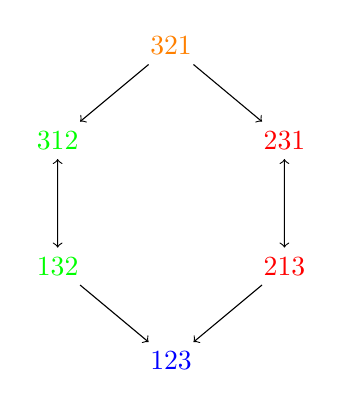
\begin{tikzpicture}[scale=0.8]
    \node [] (a123) at (0,-3) {$\color{blue}123$};
    \node [] (a132) at (-1.8,-1.5) {$\color{green}132$};
    \node [] (a213) at (1.8,-1.5) {$\color{red}213$};
    \node [] (a231) at (1.8,0.5) {$\color{red}231$};
    \node [] (a312) at (-1.8,0.5) {$\color{green}312$};
    \node [] (a321) at (0,2) {$\color{orange}321$};
    
    \draw[->] (a321) -- (a312);
    \draw[->] (a321) -- (a231);
    \draw [<->] (a312)--(a132);
    \draw [<->] (a231)--(a213);
    \draw[->] (a132) -- (a123);
    \draw[->] (a213) -- (a123);
    
    \end{tikzpicture} 
    \quad\quad
   \begin{tikzpicture}[scale=0.8]
    \node [] (a123) at (0,-2.5) {\color{blue}\ytableausetup{boxsize=1.2em}\begin{ytableau}
1 & 2 & 3 
\end{ytableau}};
    %\node [color=green] (a132) at (-1.8,-0.9) {$132$};
    %\node [color=red] (a213) at (1.8,-0.9) {$213$};
    \node [] (a231) at (1.8,-0.5) {\color{red}\begin{ytableau}
1 & 3 \\ 2 
\end{ytableau}};
    \node [] (a312) at (-1.8,-0.5) {\color{green}\begin{ytableau}
1 & 2 \\ 3 
\end{ytableau}};
    \node [] (a321) at (0,1.5) {\color{orange}\begin{ytableau}
1 \\2 \\ 3 
\end{ytableau}};
    
%    \draw (a321) -- (a312);
%     \draw (a321) -- (a231);
%   
%        \draw (a132) -- (a123);
%         \draw (a213) -- (a123);
    
    \end{tikzpicture} 

\end{center}
\caption{KL right preorder and cells. The colors represent the (right) cells.}
\label{fg:KL_cells_S3}
\end{figure}

Now if we ignore the single arrows, the `doubly' connected components are called the KL left (right) cells. Each cell induces a representation of $W$, known as the (KL) cell representation. In the case of $\sn$, each cells are indexed by a standard Young tableau $T$, and the corresponding cellular representation is the same as the irreducible representation of $\lambda=\text{shape}(T)$. Moreover, the left (resp. right) cells contain those permutations which have the same recording (resp. insertion) tableaux under the Robinson-Schensted correspondence.